\documentclass[11pt,a4paper,twocolumn]{article}

% === Core Packages ===
\usepackage[margin=2cm]{geometry}
\usepackage[utf8]{inputenc}
\usepackage[T1]{fontenc}
\usepackage{times}
\usepackage{amsmath,amssymb}
\usepackage{graphicx}
\usepackage{booktabs}
\usepackage{float}
\usepackage{enumitem}
\usepackage{tikz}
\usepackage{pgfplots}
\pgfplotsset{compat=1.18}
\usetikzlibrary{arrows.meta,shapes.geometric,positioning,calc,decorations.markings,fit,backgrounds}

% === Citation (IEEE style) ===
\usepackage[numbers,sort&compress]{natbib}
\bibliographystyle{IEEEtranN}

% === Hyperref ===
\usepackage[hidelinks]{hyperref}
\usepackage{xurl}

% === Settings ===
\setlength{\parindent}{1em}
\setlength{\parskip}{0.3em}

% === PDF metadata ===
\hypersetup{
  pdftitle={Gedecentraliseerd Reputatienetwerk: Een raamwerk voor natuurlijke maatschappelijke organisatie},
  pdfauthor={Pavel Kudrna},
  pdfsubject={Personix — a decentralized reputation network},
  pdfkeywords={Personix, decentralized reputation, reputation social network,
    decentralized identifiers, DID, meritocracy, censorship resistance},
}

% === Title ===
\title{\textbf{Gedecentraliseerd Reputatienetwerk:\\Een raamwerk voor natuurlijke maatschappelijke organisatie}}
\author{Pavel Kudrna\\Personix Project --- \url{https://personix.org}\\Prague, Czechia\\Draft v1 --- March 2026}
\date{}

\begin{document}
\maketitle

% ============================================================
% ABSTRACT
% ============================================================
\begin{abstract}
Het rechtvaardigheidsgevoel---de overtuiging dat onrecht wordt rechtgezet en verdienste wordt beloond---is de sterkste bindende kracht van de samenleving. Wanneer gecentraliseerde bestuursinstellingen dit gevoel niet kunnen leveren omdat de kosten van het afdwingen van een recht de waarde van het recht zelf overstijgen, brokkelt de maatschappelijke samenhang af. Bestaande institutionele structuren slagen er niet in een aanzienlijke categorie geschillen op te lossen, en wel op systematisch dezelfde wijze waarop centrale planning faalt bij het toewijzen van middelen: door informatieasymmetrie, ontbrekende terugkoppelingslussen en de loskoppeling van besluitvormers van de gevolgen van hun beslissingen. Dit artikel presenteert een Reputatie Sociaal Netwerk (RSN): een gedecentraliseerde, onomkoopbare, censuurbestendige communicatielaag gebouwd op Decentralized Identifiers (DIDs) die pseudonieme deelnemers in staat stelt reputatie-informatie over gedrag in de echte wereld te publiceren, te verifiëren en te consumeren. Het kernmechanisme rust op drie ontwerpprincipes: (1)~een asymmetrische kostenstructuur waarbij het lezen van reputatiegegevens goedkoop is maar het schrijven verifieerbare inspanning vereist; (2)~een niet-deterministisch protocol voor de selectie van verifieerders op basis van consistent hashing dat radicale beweringen beprijst via oplopende iteratiekosten; en (3)~een marktgedreven model van reputatie-autoriteiten waarbij private verifieerders hun opgebouwde reputatie inzetten voor de juistheid van de beweringen die zij onderschrijven. De resulterende architectuur brengt een emergente meritocratie voort zonder centrale coördinatie en maakt een geleidelijk, omkeerbaar migratiepad mogelijk vanuit bestaande, door de staat beheerde systemen.
\end{abstract}

% ============================================================
% 1. INTRODUCTION
% ============================================================
\section{Inleiding}

\subsection{Het probleem van gecentraliseerd vertrouwen}

Modern bestuur rust op een fundamentele aanname: dat gecentraliseerde instellingen op schaal vertrouwen tussen vreemden kunnen bemiddelen. Rechtbanken beslechten geschillen. Registers certificeren eigendom. Toezichthoudende instanties handhaven normen. Deze instellingen werden ontworpen in een tijdperk waarin informatie schaars was, communicatie traag verliep en de delegatie van bevoegdheid aan een centraal orgaan het enige haalbare coördinatiemechanisme was. Gecentraliseerd bestuur faalt echter om dezelfde structurele redenen als centrale planning: informatieasymmetrie, ontbrekende terugkoppelingslussen en de loskoppeling van besluitvormers van de gevolgen van hun beslissingen.

De aanname faalt bijvoorbeeld wanneer de kosten van institutionele bemiddeling de waarde van het geschil overstijgen. Neem een huurder die ontdekt dat zijn gehuurde appartement een wettelijk verplicht elektrisch veiligheidscertificaat mist---een omstandigheid die onmiddellijk levensgevaar oplevert. Het wettelijke recht van de huurder om de overeenkomst te ontbinden is ondubbelzinnig. Toch overstijgen de kosten van het afdwingen van dat recht via de rechtbank de geldwaarde van de borg en de verschuldigde schadevergoeding, zelfs met inbegrip van eventuele wettelijke compensatie~\cite{czcourtfees}. De rationele reactie is het verlies te dragen en te vertrekken.

Dit is geen pathologisch randgeval. Het is de standaardervaring voor een aanzienlijke categorie geschillen waarin de schade reëel is maar de financiële inzet onder de drempel valt waarboven institutionele handhaving economisch rationeel wordt. Het resultaat is een systeem dat structureel kwaadwillenden bevoordeelt: wie anderen schade toebrengt in hoeveelheden onder deze drempel kan ongestraft handelen, omdat de kosten van het zoeken naar recht op de benadeelde partij drukken.

Het bovenstaande voorbeeld is ontleend aan de juridische omgeving van de auteur---het Tsjechische civielrechtelijke stelsel. In andere rechtstradities---op precedenten gebaseerd common law, gewoonterecht, gemengde stelsels---faalt de rechtvaardigheid op andere manieren en in verschillende mate, afhankelijk van de culturele en procedurele bijzonderheden van het rechtsgebied. Lezers zullen waarschijnlijk gelijkwaardige voorbeelden uit hun eigen context herkennen. Wat structureel universeel is, is het patroon: geschillen waarvan de waarde onder de drempel van economisch rationele handhaving valt, eindigen ermee dat het verlies door de benadeelde partij wordt gedragen. Het RSN belooft geen perfecte rechtvaardigheid---het vermindert slechts het structurele voordeel dat kwaadwillenden genieten wanneer institutionele handhaving oneconomisch is.

\subsection{Waarom bestaande oplossingen tekortschieten}

\textbf{Raamwerken voor gedecentraliseerde identiteit (DID)}~\cite{did2022} bieden cryptografische mechanismen voor zelfsoeverein identiteitsbeheer, maar richten zich hoofdzakelijk op identiteitsverificatie zonder de bredere kwestie van gedragsreputatie aan te pakken.

\textbf{Soulbound Tokens (SBTs)}~\cite{weyl2022} vatten het inzicht dat reputatie niet-overdraagbaar is, maar leunen op blockchain-infrastructuur met schaalbaarheidsbeperkingen en pakken de economische prikkels die de invoer van informatie beheersen niet aan. Verwante concepten zoals merit tokens (bijv. Liberland) delen een vergelijkbare filosofie, maar blijven gebonden aan specifieke jurisdictionele kaders.

\textbf{Gedecentraliseerde autonome organisaties (DAO's)}~\cite{buterin2014} implementeren bestuur via smart contracts, maar reproduceren plutocratische dynamieken waarbij invloed evenredig is aan kapitaal. Quadratic voting~\cite{buterin2019} verzacht dit gedeeltelijk, maar beperkt de praktische toepassing. DAO's staan ook voor het fundamentele \emph{oracle-probleem}: smart contracts kunnen toestanden in de echte wereld niet betrouwbaar verifiëren zonder een vertrouwde externe bron, en dit probleem heeft geen algemene oplossing binnen de blockchain-architectuur.

Geen enkel bestaand systeem combineert decentralisatie, censuurbestendigheid, pseudonimiteit, verifieerbare toegangskosten en emergente consensus.

\subsection{Bijdragen}

Dit artikel levert de volgende bijdragen:
\begin{enumerate}[nosep]
\item Definitie van het \textbf{Reputatie Sociaal Netwerk (RSN)}, een gedecentraliseerd protocol dat het DID-raamwerk uitbreidt ter ondersteuning van bilaterale reputatie-uitwisseling.
\item Een \textbf{niet-deterministisch protocol voor de selectie van verifieerders} op basis van consistent hashing~\cite{karger1997}.
\item Het \textbf{principe van duur radicalisme}, dat beweringen beprijst naar hun afstand tot de netwerkconsensus via drie samenwerkende kostenkanalen.
\item Een \textbf{model van reputabele autoriteiten} met asymmetrische prikkels waarbij valse onderschrijving catastrofaal veel meer kost dan legitieme vergoedingen.
\item Een \textbf{geleidelijk migratiepad} via parallelle fiscale infrastructuur.
\end{enumerate}

% ============================================================
% 2. DESIGN PRINCIPLES
% ============================================================
\section{Ontwerpprincipes}

De RSN-architectuur wordt begrensd door vijf niet-onderhandelbare ontwerpprincipes.

\textbf{Continuïteit en evolutie.} Het systeem bestaat naast bestaande instellingen gedurende een overgangsperiode van onbepaalde duur. De overgang moet in elke fase omkeerbaar zijn.

\textbf{Vrijwilligheid en verantwoordelijkheid.} Deelname is vrijwillig, maar vrijwilligheid gaat gepaard met verantwoordelijkheid: een deelnemer die de controle over een institutionele functie op zich neemt, neemt tegelijkertijd de bijbehorende verplichtingen op zich.

\textbf{Diversiteit en culturele neutraliteit.} Consensus ontstaat uit bilaterale interacties, niet uit vooraf vastgelegde regels die door systeemontwerpers worden opgelegd.

\textbf{Veerkracht en censuurbestendigheid.} De kosten van het censureren van het netwerk moeten de kosten van het tolereren ervan overstijgen. Alleen volledig totalitarisme---tegen ruïneuze politieke en economische kosten---kan het systeem onderdrukken.

\textbf{Consensus en handhaving.} Het systeem verwerkt menselijke neigingen tot kleingeestigheid, wrok en vergeldende genoegdoening als dragende kenmerken. Wangedrag wordt niet verboden; het wordt beprijsd.

% ============================================================
% 3. SYSTEM OVERVIEW
% ============================================================
\section{Systeemoverzicht}

\subsection{Reputatie Sociaal Netwerk}

Het RSN is een gedecentraliseerde, peer-to-peer communicatielaag waarin deelnemers verifieerbare informatie over gedrag in de echte wereld uitwisselen. De bepalende eigenschappen zijn: gedecentraliseerde en niet-censureerbare infrastructuur; pseudonieme deelname via DIDs; asymmetrische kostenstructuur (lezen is goedkoop, schrijven is duur); cryptografische verifieerbaarheid; en \textbf{ondersteuning van standaarden}---machinaal leesbare formaten voor informatie die door het netwerk wordt verspreid, voor diensten die door autoriteiten worden aangeboden (samenstelling van beweringen, onderschrijving, getuigedienst) en voor het beleidsformaat, met inbegrip van regels voor het beoordelen van de reputatie van tegenpartijen en het inschatten van het risico op beleidsdiscrepantie (tussen aangegeven en werkelijk gedrag).

\subsection{Architectuurcomponenten}

Het RSN bestaat uit vier primaire componenten (Fig.~\ref{fig:architecture}):
\begin{enumerate}[nosep]
\item \textbf{DID-laag.} Identiteiten van deelnemers met aangegeven regels, reputatiemetadata en netwerkrouting.
\item \textbf{Bewering-protocol.} Gestructureerd formaat voor het publiceren van beweringen over gebeurtenissen in de echte wereld.
\item \textbf{Verificatienetwerk.} Gedecentraliseerd protocol voor het toewijzen van verifieerders via consistent hashing.
\item \textbf{Reputatie-aggregatielaag.} Diensten die voor mensen leesbare reputatiesamenvattingen produceren.
\end{enumerate}

\begin{figure}[ht]
\centering
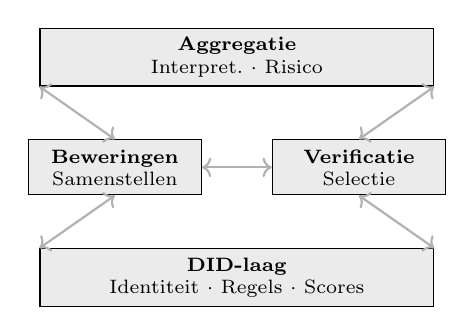
\begin{tikzpicture}[
    layer/.style={draw, minimum height=0.7cm, align=center, font=\scriptsize, fill=black!8},
    arr/.style={<->, thick, gray!60}
]
\node[layer, minimum width=5cm] (agg) at (0,2.8) {\textbf{Aggregatie}\\Interpret.\ $\cdot$ Risico};
\node[layer, minimum width=2.2cm] (claim) at (-1.55,1.4) {\textbf{Beweringen}\\Samenstellen};
\node[layer, minimum width=2.2cm] (verif) at (1.55,1.4) {\textbf{Verificatie}\\Selectie};
\node[layer, minimum width=5cm] (did) at (0,0) {\textbf{DID-laag}\\Identiteit $\cdot$ Regels $\cdot$ Scores};

\draw[arr] (agg.south west) -- (claim.north);
\draw[arr] (agg.south east) -- (verif.north);
\draw[arr] (claim.east) -- (verif.west);
\draw[arr] (claim.south) -- (did.north west);
\draw[arr] (verif.south) -- (did.north east);
\end{tikzpicture}
\caption{RSN-architectuur met vier lagen.}
\label{fig:architecture}
\end{figure}

\subsection{Rollen van deelnemers}

Een verificatietransactie omvat tot zes onderscheiden DID-rollen (Fig.~\ref{fig:roles}): \textbf{Uitgever} ($DID_I$, stelt de bewering op en dient deze in), \textbf{Onderwerp} ($DID_S$, de DID waarover de bewering gaat---kan samenvallen met de Uitgever), \textbf{Autoriteit} ($DID_A$, onderschrijft de bewering tegen een vergoeding; kan ook getuigediensten aanbieden---\emph{optioneel}), \textbf{Getuige} ($DID_{W_{1..n}}$, incognito toezichthouder op de eerlijkheid van de verifieerder via challenge-codes---\emph{optioneel}), \textbf{Verifieerder} ($DID_V$, algoritmisch geselecteerd om de bewering te publiceren) en het \textbf{RSN} (het netwerk waar geverifieerde beweringen worden gepubliceerd). Elke rol kan aan een andere DID worden gedelegeerd (Sectie~7.4). Een Autoriteit combineert doorgaans onderschrijving met getuigediensten, maar de twee functies zijn logisch onafhankelijk.

\begin{figure}[ht]
\centering
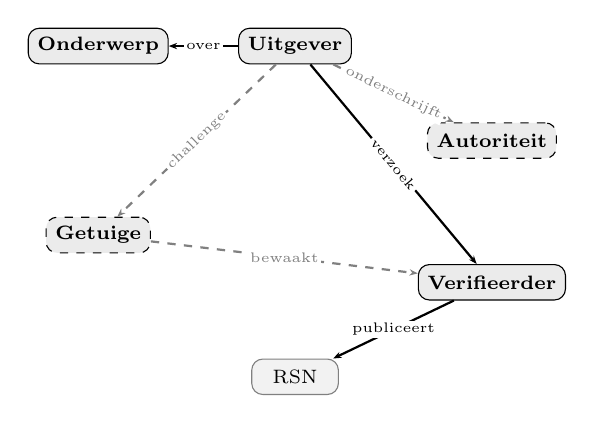
\begin{tikzpicture}[
    role/.style={draw, rounded corners, minimum width=1.1cm, minimum height=0.45cm, align=center, font=\scriptsize, fill=black!8},
    opt/.style={draw, rounded corners, minimum width=1.1cm, minimum height=0.45cm, align=center, font=\scriptsize, fill=black!8, dashed},
    arr/.style={-{Stealth[length=3pt]}, thick},
    oarr/.style={-{Stealth[length=3pt]}, thick, dashed, gray},
    lbl/.style={font=\tiny, fill=white, inner sep=1pt}
]
\node[role] (I) at (0,2.4) {\textbf{Uitgever}};
\node[role] (S) at (-2.5,2.4) {\textbf{Onderwerp}};
\node[opt] (A) at (2.5,1.2) {\textbf{Autoriteit}};
\node[opt] (W) at (-2.5,0) {\textbf{Getuige}};
\node[role] (V) at (2.5,-0.6) {\textbf{Verifieerder}};
\node[role, fill=black!5, draw=gray] (N) at (0,-1.8) {RSN};

\draw[arr] (I) -- node[lbl] {over} (S);
\draw[oarr] (I) -- node[lbl,sloped] {onderschrijft} (A);
\draw[oarr] (I) -- node[lbl,sloped] {challenge} (W);
\draw[arr] (I) -- node[lbl,sloped] {verzoek} (V);
\draw[oarr] (W) -- node[lbl] {bewaakt} (V);
\draw[arr] (V) -- node[lbl] {publiceert} (N);
\end{tikzpicture}
\caption{DID-rollen in een verificatietransactie. Gestippeld = optioneel (Autoriteit, Getuige).}
\label{fig:roles}
\end{figure}

\subsection{Onomkoopbaarheid: vier krachten}

De onomkoopbaarheid van het RSN komt niet voort uit één enkel mechanisme, maar uit vier gelijktijdige krachten. Geen enkele is op zichzelf voldoende; alleen hun combinatie maakt een corruptiepoging economisch irrationeel.

\textbf{Onvoorspelbaar doelwit.} De verifieerder voor elke bewering wordt niet-deterministisch geselecteerd via consistent hashing (Sectie~5.3). Een aanvaller kan geen specifieke verifieerder vooraf als doelwit voor omkoping kiezen, omdat de identiteit van de verifieerder een functie is van de inhoud van de bewering en van voorgaande iteraties, niet van de keuze van de uitgever.

\textbf{Reputatiehefboom---langzaam omhoog, snel omlaag.} Reputatie kan alleen stapsgewijs worden opgebouwd, via aanhoudend consistent gedrag. Ze kan echter catastrofaal verloren gaan bij één frauduleuze onderschrijving (Sectie~6.2). Deze asymmetrie betekent dat jaren van opgebouwde reputatie door één oneerlijke onderschrijving vernietigd kunnen worden; de optimale strategie blijft verdachte beweringen te weigeren.

\textbf{Publieke belofte.} Elke DID-houder verklaart publiekelijk zijn beleid---een machinaal leesbare set regels die hij zich verbindt na te leven. Afwijking tussen de verklaring en het werkelijke gedrag is detecteerbaar en wordt beprijsd als een reputatievergrijp dat ernstiger is dan de onderliggende overtreding (Sectie~7.3). Hypocrisie is daarom duurder dan directe oneerlijkheid.

\textbf{Asymmetrie van aanvalskosten in het netwerk.} De kosten van het censureren of destabiliseren van het netwerk groeien niet-lineair met de omvang en dichtheid van het netwerk, terwijl de kosten van het tolereren ervan constant blijven. Om censuur lonend te maken, zou een gecentraliseerde actor deze over het hele netwerk moeten toepassen---wat maatregelen vereist die niet in verhouding staan tot enig denkbaar voordeel (Sectie~10).

% ============================================================
% 4. DECENTRALIZED IDENTITY MODEL
% ============================================================
\section{Model voor gedecentraliseerde identiteit}

\subsection{DID met bijzondere eigenschappen}

Het RSN breidt de W3C DID Core-specificatie~\cite{did2022} uit met: \textbf{Aangegeven regels} (machinaal leesbare gedragsverbintenissen), \textbf{Reputatiemetadata} (geaggregeerde gedragsscore) en \textbf{Netwerkrouting} (veranderlijke onion-gateway, los van de stabiele ringpositie).

\subsection{Levenscyclus van een bewering}

Een bewering doorloopt zes fasen (Fig.~\ref{fig:lifecycle}): samenstelling, optionele onderschrijving door een autoriteit, selectie van de verifieerder via consistent hashing, verificatiebeslissing (aanvaarden of weigeren met iteratie), publicatie en reputatie-update voor alle partijen.

\begin{figure}[ht]
\centering
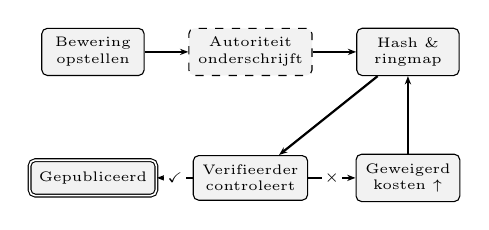
\begin{tikzpicture}[
    stp/.style={draw, rounded corners=2pt, minimum width=1.3cm, minimum height=0.45cm, align=center, font=\tiny, fill=black!5},
    arr/.style={-{Stealth[length=3pt]}, thick},
    lbl/.style={font=\tiny, fill=white, inner sep=1pt}
]
\node[stp] (comp) at (0,0) {Bewering\\opstellen};
\node[stp, dashed] (auth) at (2.0,0) {Autoriteit\\onderschrijft};
\node[stp] (hash) at (4.0,0) {Hash \&\\ringmap};
\node[stp] (ver) at (2.0,-1.6) {Verifieerder\\controleert};
\node[stp, double] (pub) at (0,-1.6) {Gepubliceerd};
\node[stp] (rej) at (4.0,-1.6) {Geweigerd\\kosten $\uparrow$};

\draw[arr] (comp) -- (auth);
\draw[arr] (auth) -- (hash);
\draw[arr] (hash) -- (ver);
\draw[arr] (ver) -- node[lbl] {\checkmark} (pub);
\draw[arr] (ver) -- node[lbl] {$\times$} (rej);
\draw[arr] (rej) -- ++(0,0.8) -| (hash);
\end{tikzpicture}
\caption{Levenscyclus van een bewering met iteratielus.}
\label{fig:lifecycle}
\end{figure}

\subsection{Relatie tot W3C DID Core}

Het identiteitsmodel van het RSN is een echte superset van de W3C DID Core-specificatie~\cite{did2022}. Alle RSN-DIDs zijn geldige W3C-DIDs. De RSN-specifieke uitbreidingen zijn gecodeerd als eigenschappen van het DID-document, gedefinieerd in een specifieke DID-methodespecificatie, compatibel met bestaande infrastructuur zoals ION~\cite{buchner2021} en Ceramic~\cite{ceramic2023}.

% ============================================================
% 5. VERIFICATION AND PROPAGATION
% ============================================================
\section{Verificatie en verspreiding van informatie}

\subsection{Kosten van informatie-invoer}

Het economische kernprincipe van het RSN is de asymmetrie tussen lezen en schrijven. Het lezen van reputatiegegevens nadert nulmarginale kosten voor deelnemers die deel uitmaken van het DID-netwerk en toegang hebben die in verhouding staat tot hun reputatie---nieuwkomers moeten geleidelijk bredere toegang verdienen (zie anti-leeching). Schrijven---opgevat als de duurzame materialisatie van reputatie in het netwerk, niet als een eenmalige technische handeling---vereist een verifieerbare cumulatieve investering langs drie dimensies: \textbf{tijd} (levensjaren besteed aan consistent gedrag, nagekomen verbintenissen en gecultiveerde relaties), \textbf{energie} (inspanning geïnvesteerd in eerlijk handelen, zorg voor samenwerkingen en betrouwbaarheid op lange termijn) en \textbf{geld} (investering in de eigen naam---professionele ontwikkeling, de kwaliteit van het eigen werk, herstel van veroorzaakte schade). Reputatie kan niet onmiddellijk worden gekocht---ze is het resultaat van levenslange opbouw die het systeem slechts zichtbaar en overdraagbaar tussen contexten maakt. De eenmalige technische kosten van het protocol (cryptografische handtekeningen, vergoedingen voor verifieerders) zijn verwaarloosbaar in vergelijking met deze onderliggende investering.

\subsection{Sociale grafiek en contactdiepte}

Het RSN is fundamenteel een sociaal netwerk: elke DID voegt contacten toe (andere DIDs) die de verbinding toestaan. Deze contacten hebben hun eigen contacten, enzovoort. De algoritmische zoektocht naar verifieerders werkt binnen een instelbare diepte $h$ van gekoppelde contacten (bijv. $h=3$: de eigen directe contacten, hun contacten, en contacten van contacten). Deze architectuur vereist geen enkele wereldwijde blockchain---ze bevordert van nature het ontstaan van gemeenschappen/clusters met overlappingen naar andere gemeenschappen. Elke DID-deelnemer moet een gepubliceerd \textbf{beleid} hebben---een machinaal leesbare set regels die bepaalt hoe inkomende verzoeken worden beoordeeld. Beleidsschendingen worden als negatieve artefacten in het netwerk vastgelegd.

\subsection{Algoritmische selectie van verifieerders}

Het verificatieprotocol maakt gebruik van consistent hashing~\cite{karger1997} (Fig.~\ref{fig:verifier}). Verificatie is een betaalde dienst: verifieerders werken tegen een vergoeding, wat een markt creëert waarin concurrentie prijsstelling, snelheid en betrouwbaarheid aandrijft.

\textbf{Stap 1.} Het beweringsdocument wordt samengevoegd met het hashresultaat van de vorige iteratie (of $\varnothing$ bij de eerste iteratie) en gehasht:
\begin{equation}
\text{pos} = f_h(\text{claim} \| \text{prev\_hash})
\label{eq:hash}
\end{equation}

Het algoritme moet het \emph{volledige pad} van alle voorgaande verzoeken en antwoorden bevatten---niet louter een hash van de vorige iteratie. Het volledige antwoord van elke verifieerder (aanvaarding, weigering, opgegeven prijs, reden) wordt aan het groeiende document toegevoegd, verifieerbaar via cryptografische handtekeningen bij elke stap.

\textbf{Stap 2.} De hash wordt afgebeeld op $N$ posities op de consistent-hashring, gelijkmatig verdeeld (bijv. voor $N=4$: $+0^{\circ}, +90^{\circ}, +180^{\circ}, +270^{\circ}$). Vanaf elke positie selecteert een zoektocht met de klok mee de dichtstbijzijnde DID als kandidaat-verifieerder (Fig.~\ref{fig:multipoint}). $N$ is een variabele parameter die kan afhangen van het percentage momenteel actieve DIDs, het tijdstip van de dag of de historische reactiesnelheid van het netwerk.

\textbf{Stap 3.} De Verifieerder aanvaardt (publiceert en zet reputatie in) of weigert (keert terug naar Stap~1 met de weigeringshash). Wanneer een knooppunt niet reageert ondanks een verklaarde online-status, moet het volgende verzoek alle antwoorden van alle $N$ voorgaande kandidaat-verifieerders bevatten.

\textbf{Anti-leeching.} Doel-DIDs mogen vergoedingen of toegangsbeperkingen instellen voor vragen van nieuwe DIDs met weinig reputatie. Dit gegradeerde mechanisme (niet binair) dwingt nieuwkomers reputatie op te bouwen door echte activiteit voordat zij vrijelijk de gegevens van anderen consumeren.

\begin{figure}[ht]
\centering
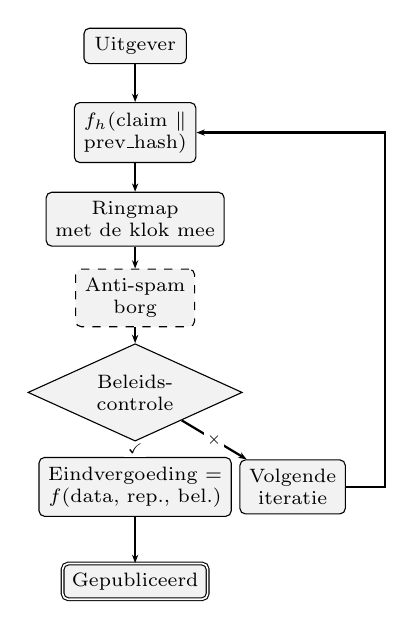
\begin{tikzpicture}[
    box/.style={draw, rounded corners=2pt, minimum width=1.3cm, minimum height=0.45cm, align=center, font=\scriptsize, fill=black!5},
    dec/.style={draw, diamond, aspect=2.2, minimum width=0.9cm, align=center, font=\scriptsize, fill=black!5},
    arr/.style={-{Stealth[length=3pt]}, thick},
    lbl/.style={font=\tiny, fill=white, inner sep=1pt}
]
\node[box] (iss) at (0,0) {Uitgever};
\node[box] (hash) at (0,-1.1) {$f_h$(claim $\|$\\prev\_hash)};
\node[box] (ring) at (0,-2.2) {Ringmap\\met de klok mee};
\node[box, dashed] (spam) at (0,-3.2) {Anti-spam\\borg};
\node[dec] (check) at (0,-4.4) {Beleids-\\controle};
\node[box] (rej) at (2,-5.6) {Volgende\\iteratie};
\node[box] (fee) at (0,-5.6) {Eindvergoeding =\\$f$(data, rep., bel.)};
\node[box, double] (pub) at (0,-6.8) {Gepubliceerd};

\draw[arr] (iss) -- (hash);
\draw[arr] (hash) -- (ring);
\draw[arr] (ring) -- (spam);
\draw[arr] (spam) -- (check);
\draw[arr] (check) -- node[lbl] {$\times$} (rej);
\draw[arr] (check) -- node[lbl] {\checkmark} (fee);
\draw[arr] (fee) -- (pub);
\draw[arr] (rej.east) -- ++(0.5,0) |- (hash.east);
\end{tikzpicture}
\caption{Protocol voor de selectie van verifieerders. De anti-spamborg is optioneel en kan restitueerbaar zijn. De eindvergoeding wordt alleen bij aanvaarding betaald.}
\label{fig:verifier}
\end{figure}

Elke weigering voegt het volledige antwoord van de verifieerder (inclusief redenen en voorwaarden) toe aan het beweringsdocument, waardoor de inhoud ervan uitdijt. Op basis van het uitgebreide document wordt niet-deterministisch een nieuwe hash berekend, die naar een andere ringpositie wijst en een andere verifieerder selecteert. Documentatie van het volledige pad is verplicht---de uitgever kan de volgende verifieerder niet voorspellen of beïnvloeden. Als een verifieerder een verzoek negeert ondanks een compatibel verklaard beleid, leggen getuigen (indien aanwezig) dit vast, en de uitgever kan getuigenbewijs bijvoegen bij de uiteindelijke publicatie.

\begin{figure}[ht]
\centering
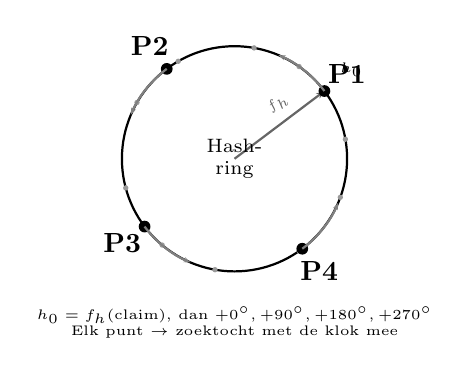
\begin{tikzpicture}[scale=0.65]
% Ring
\draw[thick] (0,0) circle (2.2cm);
% DID nodes on ring
\foreach \a in {10,55,80,120,150,195,230,260,305,340} {
  \fill[black!40] (\a:2.2) circle (1.5pt);
}
% Hash offset arrow pointing to initial position
\draw[-{Stealth[length=3pt]}, thick, black!60] (0,0) -- node[font=\tiny,above,sloped,pos=0.6] {$f_h$} (37:2.2);
\fill[black] (37:2.2) circle (2pt);
\node[font=\tiny,anchor=south west] at (37:2.35) {$h_0$};
% N=4 points offset from h0 by +0, +90, +180, +270
\foreach \offset/\l in {0/P1,90/P2,180/P3,270/P4} {
  \pgfmathsetmacro{\ang}{37+\offset}
  \node[fill=black, circle, inner sep=1.5pt] (p\offset) at (\ang:2.2) {};
  \node[font=\tiny,font=\bfseries] at (\ang:2.75) {\l};
  % clockwise search arc
  \draw[-{Stealth[length=2.5pt]}, thick, gray] (\ang:2.2) arc (\ang:\ang+30:2.2);
}
\node[font=\scriptsize, align=center] at (0,0) {Hash-\\ring};
\node[font=\tiny, align=center] at (0,-3.2) {$h_0 = f_h(\text{claim})$, dan $+0^{\circ},+90^{\circ},+180^{\circ},+270^{\circ}$\\Elk punt $\rightarrow$ zoektocht met de klok mee};
\end{tikzpicture}
\caption{Selectie op meerdere punten ($N{=}4$). Hash $h_0$ bepaalt de verschuiving; 4 punten gelijkmatig verdeeld vanaf $h_0$.}
\label{fig:multipoint}
\end{figure}

\subsection{Getuigeprotocol}

De rol van \textbf{Getuige} biedt incognito verantwoording voor de eerlijkheid van de verifieerder via een cryptografisch challenge-code-protocol:

\textbf{Stap W1.} De verzoeker ondertekent het verificatieverzoek en verzendt het naar $N_w$ getuigen---contacten uit het sociale netwerk van de verzoeker, of gespecialiseerde aanbieders van getuigediensten die tegen een vergoeding werken.

\textbf{Stap W2.} Elke getuige $w_i$ ondertekent het volledige ondertekende verzoek, behoudt de oorspronkelijke handtekening $\sigma_i$ en berekent een challenge-code $c_i = h(\sigma_i)$. De challenge-code wordt aan het verzoek toegevoegd.

\textbf{Stap W3.} Het verzoek, dat nu $N_w$ challenge-codes draagt, wordt naar de verifieerder verzonden. De verifieerder ziet de codes maar \emph{kan niet vaststellen} wie de getuigen zijn of dat de codes overeenkomen met echte handtekeningen.

\textbf{Stap W4 (eerlijke verifieerder).} Als de verifieerder reageert volgens zijn verklaarde beleid, blijven de challenge-codes ondoorzichtig. Getuigen worden nooit onthuld. Er worden geen aanvullende gegevens gepubliceerd.

\textbf{Stap W5 (beleidsschending).} Als de verifieerder zijn beleid schendt (het verzoek negeert, inconsistent reageert), bezit de verzoeker de oorspronkelijke handtekeningen $\sigma_i$ van de getuigen. Deze kunnen als begeleidende gegevens worden gepubliceerd: iedereen kan $c_i = h(\sigma_i)$ verifiëren, wat bewijst dat de getuige aanwezig was. De verzoeker kan onafhankelijk publiceren---de verifieerder heeft de challenge-codes al in zijn antwoord ondertekend.

\textbf{De bluf-eigenschap.} De verzoeker mag willekeurige waarden invullen voor sommige of alle challenge-codes. De verifieerder kan echte codes (gedekt door hoogaangeschreven autoriteiten) niet van ruis onderscheiden. Deze \emph{onzekerheid} is het handhavingsmechanisme: elk verzoek draagt het risico dat een gerespecteerde autoriteit incognito meekijkt. De kosten van het handhaven van deze druk zijn vrijwel nul (het genereren van willekeurige getallen), terwijl de mogelijke kosten van oneerlijkheid voor de verifieerder catastrofaal zijn. Eerlijk gedrag wordt aangemoedigd, zelfs bij afwezigheid van werkelijke getuigen.

\textbf{Autoriteit als getuige.} Een Autoriteit die een bewering onderschrijft, mag getuigediensten bundelen: ``Ik onderschrijf uw bewering en dien als incognito getuige tijdens de verificatie.'' Dit is een natuurlijk bedrijfsmodel---de Autoriteit beschikt al over de context. De twee rollen zijn echter logisch onafhankelijk.

\subsection{Principe van duur radicalisme}

Drie kostenkanalen versterken elkaar gelijktijdig (Fig.~\ref{fig:radicalism}):

\textbf{Kanaal 1: iteratiekosten.} Elke weigering dwingt een nieuwe iteratie af die tijd en middelen verbruikt. Lineaire groei.

\textbf{Kanaal 2: documentopzwelling.} Elke iteratie voegt het volledige antwoord van de verifieerder toe aan het beweringsdocument. De groei is lineair, maar met een basisverschuiving: de initiële payload (inhoud van de bewering, onderschrijving door de autoriteit, cryptografische handtekeningen) heeft al een niet-triviale omvang $B_0$. Totale omvang na $k$ iteraties: $S(k) = B_0 + k \cdot \Delta$, waarbij $\Delta$ de gemiddelde antwoordomvang is.

\textbf{Kanaal 3: risicopremie van de verifieerder.} Risico is subjectief. De verifieerder beoordeelt of het verklaarde beleid van de verzoekende DID in conflict is met zijn eigen commerciële, sociale of politieke belangen. De premie kan exponentieel oplopen met de waargenomen afstand tot het ``ideaal'' van de verifieerder: $P(d) = \alpha \cdot e^{\beta d}$, waarbij $d$ de subjectieve afstandsmaat van de verifieerder is. Voorbij een persoonlijke no-go-grens mag de verifieerder volledig weigeren.

\begin{figure}[ht]
\centering
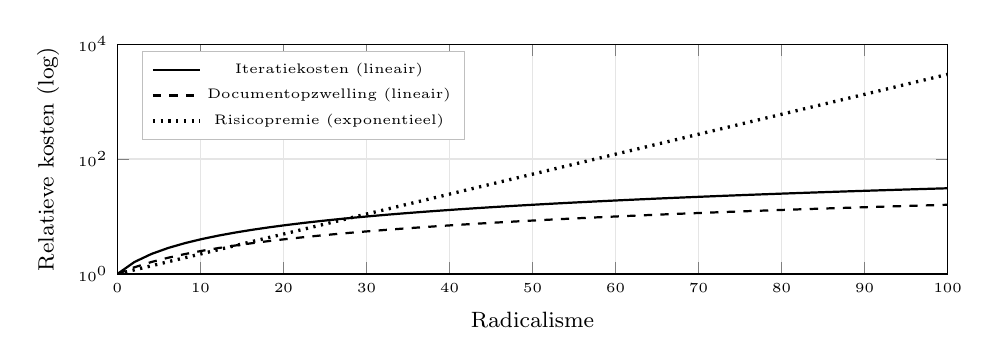
\begin{tikzpicture}
\begin{axis}[
    width=\columnwidth,
    height=4.5cm,
    xlabel={\footnotesize Radicalisme},
    ylabel={\footnotesize Relatieve kosten (log)},
    ymode=log,
    xmin=0, xmax=100,
    ymin=1, ymax=10000,
    grid=major,
    grid style={gray!20},
    legend style={at={(0.03,0.97)},anchor=north west,font=\tiny,draw=gray!50},
    tick label style={font=\tiny},
    label style={font=\footnotesize},
]
\addplot[black, thick, domain=0:100, samples=50] {1 + 0.3*x};
\addlegendentry{Iteratiekosten (lineair)}
\addplot[black, thick, dashed, domain=0:100, samples=50] {1 + 0.15*x};
\addlegendentry{Documentopzwelling (lineair)}
\addplot[black, thick, dotted, line width=1.2pt, domain=0:100, samples=100] {exp(0.08*x)};
\addlegendentry{Risicopremie (exponentieel)}
\end{axis}
\end{tikzpicture}
\caption{Kostenescalatie over drie kanalen. De risicopremie domineert bij hoog radicalisme.}
\label{fig:radicalism}
\end{figure}

Cruciaal is dat dit geen censuur is. Geen enkele bewering wordt verboden. Het systeem beprijst risico (Tabel~\ref{tab:costs}).

\begin{table}[ht]
\centering
\caption{Kostenvergelijking over verschillende soorten beweringen.}
\label{tab:costs}
\footnotesize
\begin{tabular}{@{}lcccc@{}}
\toprule
\textbf{Type} & \textbf{Iter.} & \textbf{Doc} & \textbf{Verg.} & \textbf{Totaal} \\
\midrule
Geloofwaardig & $k_{\min}$ & $B_0$ & $P_{\min}$ & Laag \\
Controversieel & $k_{\text{med}}$ & $B_0{+}k\Delta$ & $\alpha e^{\beta d}$ & Matig \\
Radicaal & $k_{\max}$ & $\gg B_0$ & $\gg P_{\min}$ & Zeer hoog \\
Frauduleus & $\to\infty$ & --- & --- & Onpubliceerbaar \\
\bottomrule
\end{tabular}
\end{table}

% ============================================================
% 6. REPUTATION AND RISK
% ============================================================
\section{Reputatie- en risicobeoordeling}

\subsection{Model voor reputatieopbouw}

Reputatie vertoont drie eigenschappen: \textbf{trage opbouw} (stapsgewijze groei door consistent gedrag), \textbf{snelle vernietiging} (één enkele fraude kan de score catastrofaal verlagen) en \textbf{individuele beoordeling} (elke consumerende partij mag haar eigen aggregatiefunctie toepassen).

\subsection{Reputabele autoriteiten}

Een Reputabele Autoriteit beoordeelt beweringen en medeondertekent ze als ze tevreden is---waarbij ze haar eigen reputatie inzet (Fig.~\ref{fig:authority}). De asymmetrie is opzettelijk: reputatie winnen is traag (stapsgewijs $+\delta$ per eerlijke onderschrijving), terwijl ze verliezen catastrofaal is ($-\Delta \gg \delta$ per valse onderschrijving; ter illustratie bijv. $+2\%$ tegenover $-70\%$). De optimale strategie is altijd verdachte beweringen te weigeren. De specifieke waarden van $\delta$ en $\Delta$ zijn systeemparameters.

\begin{figure}[ht]
\centering
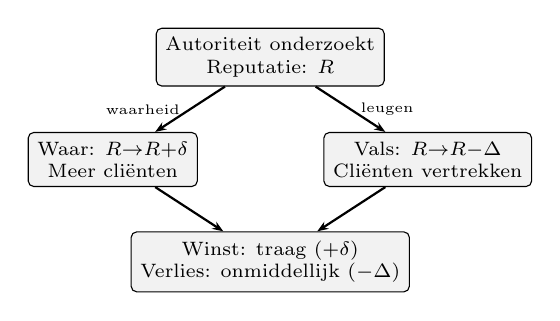
\begin{tikzpicture}[
    box/.style={draw, rounded corners=2pt, minimum width=2cm, minimum height=0.6cm, align=center, font=\scriptsize, fill=black!5},
    arr/.style={-{Stealth[length=4pt]}, thick}
]
\node[box] (exam) at (0,0) {Autoriteit onderzoekt\\Reputatie: $R$};
\node[box] (true) at (-2,-1.3) {Waar: $R{\to}R{+}\delta$\\Meer cliënten};
\node[box] (false) at (2,-1.3) {Vals: $R{\to}R{-}\Delta$\\Cliënten vertrekken};
\node[box] (insight) at (0,-2.6) {Winst: traag ($+\delta$)\\Verlies: onmiddellijk ($-\Delta$)};

\draw[arr] (exam) -- node[left,font=\tiny] {waarheid} (true);
\draw[arr] (exam) -- node[right,font=\tiny] {leugen} (false);
\draw[arr] (true) -- (insight);
\draw[arr] (false) -- (insight);
\end{tikzpicture}
\caption{Reputabele Autoriteit---asymmetrische prikkels.}
\label{fig:authority}
\end{figure}

\subsection{Multidimensionale reputatie}

Reputatie is geen scalair maar een vector over meerdere dimensies: financiële betrouwbaarheid, persoonlijke integriteit, professionele competentie, maatschappelijke betrokkenheid en andere (Fig.~\ref{fig:reputation-radar}). Verschillende evaluatie-aanbieders projecteren deze vector anders, afhankelijk van de context---een kredietverstrekker geeft voorrang aan financiële betrouwbaarheid, een werkgever aan professionele competentie, een buur aan maatschappelijk gedrag. Er bestaat geen enkele ``juiste'' reputatiescore; alleen perspectieven.

\begin{figure}[ht]
\centering
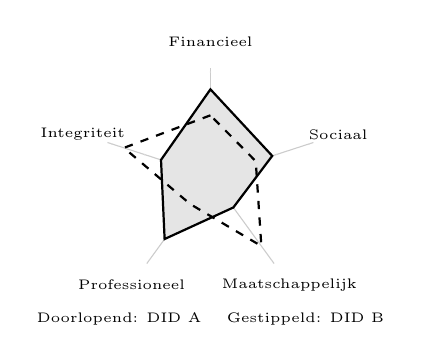
\begin{tikzpicture}[scale=0.55]
\foreach \a/\l in {90/Financieel,162/Integriteit,234/Professioneel,306/Maatschappelijk,18/Sociaal} {
  \draw[gray!40] (0,0) -- (\a:2.5);
  \node[font=\tiny, align=center] at (\a:3.1) {\l};
  \foreach \r in {0.8,1.6,2.4} {
    \fill[black!15] (\a:\r) circle (0.5pt);
  }
}
\draw[thick, fill=black!10] (90:2.0) -- (162:1.2) -- (234:1.8) -- (306:0.9) -- (18:1.5) -- cycle;
\draw[thick, dashed] (90:1.4) -- (162:2.1) -- (234:0.8) -- (306:2.0) -- (18:1.1) -- cycle;
\node[font=\tiny] at (0,-3.3) {Doorlopend: DID A \quad Gestippeld: DID B};
\end{tikzpicture}
\caption{Multidimensionale reputatievectoren. Verschillende DIDs vertonen verschillende profielen over de dimensies.}
\label{fig:reputation-radar}
\end{figure}

\subsection{Gedemocratiseerde risicobeoordeling}

Het RSN democratiseert systematische risicobeoordeling---een capaciteit die momenteel geconcentreerd is bij financiële instellingen maar veel breder toepasbaar is dan bankieren. Industriële conglomeraten die de betrouwbaarheid van leveranciers beoordelen, verzekeraars die gedragsrisico beprijzen, due diligence bij fusies en overnames, schatting van de levensduur van apparatuur in de productie---overal waar tegenpartijrisico beoordeling vereist, biedt het RSN een gedecentraliseerd, marktgedreven alternatief. Een markt van interpretatiediensten vertaalt ruwe multidimensionale reputatiegegevens in bruikbare samenvattingen, waardoor de beoordeling van tegenpartijen tegen marginale kosten toegankelijk wordt voor elke deelnemer.

% ============================================================
% 7. CONSENSUS AND DISPUTE RESOLUTION
% ============================================================
\section{Consensus en geschillenbeslechting}

\subsection{Model voor gedecentraliseerde rechtvaardigheid}

Het RSN herformuleert rechtvaardigheid als een probleem van bilaterale onderhandeling. De dreiging van permanente, verifieerbare reputatieschade is een doeltreffender afschrikmiddel dan een gerechtelijke procedure die de benadeelde partij zich niet kan veroorloven.

\subsection{Emergente consensus}

Elke deelnemer hanteert een persoonlijke tevredenheidsdrempel. De geaggregeerde consensus van het netwerk ontstaat als het statistische gemiddelde van duizenden bilaterale onderhandelingen (Fig.~\ref{fig:consensus}). Een reactie ver boven de consensus (barbaars) is duur om te publiceren. Een reactie dicht bij de consensus (evenredig) is goedkoop. De consensus is geen regel---het is een prijssignaal.

\begin{figure}[ht]
\centering
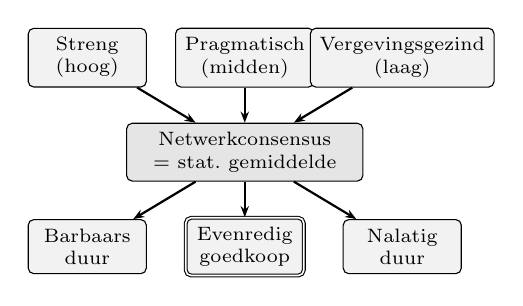
\begin{tikzpicture}[
    person/.style={draw, rounded corners=2pt, minimum width=1.5cm, minimum height=0.5cm, align=center, font=\scriptsize, fill=black!5},
    arr/.style={-{Stealth[length=4pt]}, thick}
]
\node[person] (a) at (-2,0) {Streng\\(hoog)};
\node[person] (b) at (0,0) {Pragmatisch\\(midden)};
\node[person] (c) at (2,0) {Vergevingsgezind\\(laag)};
\node[person, fill=black!10, minimum width=3cm] (cons) at (0,-1.2) {Netwerkconsensus\\= stat.\ gemiddelde};
\node[person] (exp) at (-2,-2.4) {Barbaars\\duur};
\node[person, double] (prop) at (0,-2.4) {Evenredig\\goedkoop};
\node[person] (neg) at (2,-2.4) {Nalatig\\duur};

\draw[arr] (a) -- (cons);
\draw[arr] (b) -- (cons);
\draw[arr] (c) -- (cons);
\draw[arr] (cons) -- (exp);
\draw[arr] (cons) -- (prop);
\draw[arr] (cons) -- (neg);
\end{tikzpicture}
\caption{Emergente consensus uit individuele tevredenheidsdrempels.}
\label{fig:consensus}
\end{figure}

\subsection{Kalibratie van bestraffing}

Elke DID-houder verklaart publiekelijk zijn reacties op specifieke categorieën van wangedrag. Onevenredig harde of milde verklaringen trekken negatieve reputatiesignalen aan. Evenredige verklaringen worden zonder wrijving aanvaard---een zelfkalibrerend bestraffingssysteem.

Consensusverklaringen zijn zelf onderworpen aan detectie van hypocrisie: zich declaratief verbinden aan een consensuspositie terwijl men zich inconsistent gedraagt, vormt een reputatievergrijp dat ernstiger is dan de onderliggende afwijking, aangezien het opzettelijke misleiding aantoont.

\subsection{Delegatie}

Alle activiteiten binnen een DID---met één uitzondering---mogen aan een andere DID worden gedelegeerd. \textbf{De rol van Onderwerp---de DID over wiens gedrag de bewering gaat---kan niet worden gedelegeerd; ze is niet-overdraagbaar gebonden aan de identiteitshouder op wie de bewering betrekking heeft.} De andere actieve rollen---Uitgever, Autoriteit, Getuige, Verifieerder---kunnen worden overgedragen aan een aangewezen gedelegeerde DID, hetzij voor verificatie, het indienen van beweringen, deelname aan de consensus of geschillenbeslechting. Delegatie is te allen tijde herroepbaar. Dit maakt specialisatie mogelijk (bijv. professionele verificatiediensten) terwijl de Houder de uiteindelijke controle en verantwoordelijkheid behoudt. Delegatie is van toepassing op het hele systeem en is essentieel voor schaalbaarheid.

\subsection{Van individuele moraal naar een emergent sociaal contract}

Het verklaarde beleid van elke DID vertegenwoordigt een formalisering van individuele moraal: wat de Houder aanvaardbaar acht, hoe hij reageert op specifiek gedrag, wat hij van tegenpartijen verlangt. Dit beleid wordt niet opgelegd door een systeemontwerper---het wordt door elke deelnemer gekozen en in machinaal leesbare vorm uitgedrukt.

Deze formalisering maakt een driefasige emergentie mogelijk. Ten eerste wordt individuele moraal gecodeerd als \textbf{beleid}---een set verklaarde regels, drempels en responsfuncties die de DID zich verbindt na te leven. Ten tweede brengt het geheel van alle beleidsregels in het netwerk \textbf{emergente ethiek} voort---statistisch waarneembare normen die geen enkele deelnemer heeft ontworpen maar die voortkomen uit de interactie van duizenden individuele morele posities~\cite{durkheim1893}. Ten derde vormt deze emergente ethiek, uitgedrukt als gedeelde gedragsnormen die worden gehandhaafd via bilaterale prijssignalen, een \textbf{meetbaar sociaal contract}---geen theoretisch construct dat niemand heeft ondertekend~\cite{rawls1971}, maar een empirisch waarneembare set regels die door daadwerkelijk gedrag wordt ondersteund.

Dit proces weerspiegelt bevindingen uit de moral foundations theory~\cite{haidt2012}: menselijke moraal is intuïtief, pluralistisch en cultureel variabel. Het RSN vereist geen morele consensus als input; het produceert gedragsconsensus als output. Het resulterende sociale contract is niet statisch---het evolueert naarmate deelnemers toetreden, vertrekken en hun beleid aanpassen als reactie op netwerkfeedback. In tegenstelling tot de klassieke sociaal-contracttheorie is dit contract herroepbaar, waarneembaar en afdwingbaar zonder een soeverein.

% ============================================================
% 8. ECONOMIC MODEL
% ============================================================
\section{Economisch model}

De voorgaande secties beschreven een instrument---de verificatiemechanismen, kostenstructuur en emergente consensus van het RSN. Deze sectie beschrijft een methodologie voor het toepassen van dit instrument op een fiscale en bestuurlijke overgang. Het instrument is algemeen inzetbaar; de onderstaande methodologie is één mogelijke toepassing.

\subsection{Prikkelstructuur}

Reputatie als kapitaal creëert directe prikkels voor eerlijk gedrag. In normale werking bouwen deelnemers op natuurlijke wijze reputatie op via alledaagse transacties en nagekomen verbintenissen. De voornaamste uitgave betreft \emph{negatieve} beweringen---het vastleggen van door anderen aangerichte schade. Deze asymmetrie stimuleert nuttig, betrouwbaar gedrag: eerlijk zijn kost niets extra, terwijl schadelijk zijn een gedocumenteerd spoor achterlaat dat anderen zullen betalen om te bewaren. Hypocrisie---regels verklaren zonder ze na te leven---is de duurste faalwijze, aangezien het opzettelijke misleiding aantoont.

\subsection{Parallel fiscaal systeem}

Drie componenten maken concurrentiedruk mogelijk: (1)~\textbf{Eenvoudige belasting}---één enkel proportioneel tarief zonder uitzonderingen, aanvankelijk marginaal onder het bestaande effectieve tarief; (2)~\textbf{Elektronische uitgavenregistratie (ESR)}---een omkering van het Tsjechische EET-model zodat burgers de staatsuitgaven bewaken; (3)~\textbf{Door burgers gestuurde belastingtoewijzing}---beginnend bij enkele procenten in het eerste jaar en na een decennium ergens tussen de lage dubbele cijfers en een volledige migratie naar een door burgers gestuurd systeem, afhankelijk van de mate van adoptie. Het werkelijke tempo hangt af van de snelheid waarmee vrijemarktalternatieven voor staatsdiensten ontstaan en van de bereidheid van de staat om aan de overgang mee te werken; de functie van de tijd hoeft niet lineair te zijn, en er is geen reden om een bovengrens te stellen aan waar de adoptie uiteindelijk kan uitkomen.

% ============================================================
% 9. MIGRATION PATH
% ============================================================
\section{Migratiepad}

De migratie verloopt via drie fasen (Fig.~\ref{fig:migration}): \textbf{Fase~1: overlay} (RSN als informatielaag, de staat is de enige aanbieder), \textbf{Fase~2: concurrentie} (RSN biedt functionele alternatieven, gebruik van beide systemen) en \textbf{Fase~3: overgang} (RSN presteert beter dan de staatsequivalenten, vrijwillige migratie). De overgang is in elke fase omkeerbaar.

\begin{figure}[ht]
\centering
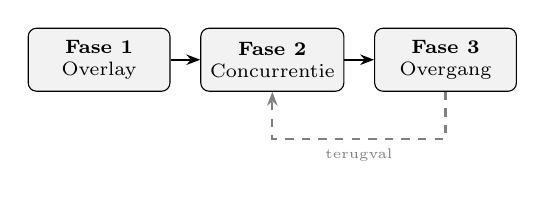
\begin{tikzpicture}[
    phase/.style={draw, rounded corners=3pt, minimum width=1.8cm, minimum height=0.8cm, align=center, font=\scriptsize, fill=black!5},
    arr/.style={-{Stealth[length=5pt]}, thick}
]
\node[phase] (p1) at (0,0) {\textbf{Fase 1}\\Overlay};
\node[phase] (p2) at (2.2,0) {\textbf{Fase 2}\\Concurrentie};
\node[phase] (p3) at (4.4,0) {\textbf{Fase 3}\\Overgang};

\draw[arr] (p1) -- (p2);
\draw[arr] (p2) -- (p3);
\draw[arr, dashed, gray] (p3.south) -- ++(0,-0.6) -| node[below,font=\tiny,pos=0.25] {terugval} (p2.south);
\end{tikzpicture}
\caption{Migratie in drie fasen---in elke fase omkeerbaar.}
\label{fig:migration}
\end{figure}

Het voornaamste drukmechanisme is fiscaal: wanneer voorwaardelijke belastingbetalers een ``economisch significante minderheid $X$'' bereiken---een groep die groot genoeg is dat repressie ertegen niet-triviale economische schade veroorzaakt en burgerlijke ongehoorzaamheid een geloofwaardige dreiging wordt---treedt de staat in onderhandeling. Ter illustratie gebruiken we $X \approx 15\%$ van het bbp, maar de werkelijke drempel hangt af van de specifieke economie.

% ============================================================
% 10. SECURITY ANALYSIS
% ============================================================
\section{Veiligheidsanalyse}

We beschouwen vijf categorieën van tegenstanders: individuele kwaadwillenden, georganiseerde groepen, bedrijfsmatige tegenstanders, tegenstanders op statelijk niveau en tegenstanders op protocolniveau.

\textbf{Sybil-bestendigheid}~\cite{douceur2002}. Het opbouwen van reputatie vereist aanhoudende, verifieerbare interactie. De kosten van een geslaagde Sybil-aanval schalen lineair met het aantal valse identiteiten en kwadratisch met het beoogde reputatieniveau. Meerdere DIDs parallel bedienen is mogelijk maar bewust duur---elke identiteit moet onafhankelijk reputatie opbouwen door echte activiteit. In vrije samenlevingen schrikt deze kostprijs terloops misbruik af; in dictaturen worden parallelle DIDs een overlevingsinstrument dat gecompartimenteerd verzet, ondergrondse coördinatie en veiliger navigatie op de zwarte markt mogelijk maakt.

\textbf{Verdediging tegen collusie.} Patronen van wederzijdse onderschrijving binnen gesloten groepen zijn detecteerbaar via analyse van de sociale grafiek. Reputatie-aggregatiefuncties verdisconteren beweringen uit sterk geclusterde bronnen.

\textbf{Tegenstander op statelijk niveau.} Onion-routing, de afwezigheid van gecentraliseerde infrastructuur en de verdeling van de rol van Verifieerder over de deelnemersbasis waarborgen dat onderdrukking maatregelen vereist die niet in verhouding staan tot enig voordeel.

\textbf{Privacy tegenover verantwoording.} Pseudonimiteit---een tussenweg tussen anonimiteit en identiteitsonthulling---stelt DIDs in staat betekenisvolle reputatie op te bouwen zonder de reële identiteit van de Houder te onthullen.

% ============================================================
% 11. PRIVACY
% ============================================================
\section{Privacyoverwegingen}

Het privacymodel van het RSN is gebouwd op pseudonimiteit. De Houder bepaalt de openbaarmaking van identiteit: minimaal (zuiver pseudoniem), selectief (specifieke referenties gekoppeld) of volledig (wettelijke identiteit gekoppeld). Gepubliceerde beweringen zijn permanent---het systeem ondersteunt contextuele correctie maar geen wissing. Een Houder mag een gecompromitteerde DID opgeven en opnieuw beginnen, waarbij hij de opgebouwde reputatie prijsgeeft.

% ============================================================
% 12. RELATED WORK
% ============================================================
\section{Verwant werk}

De W3C DID Core-specificatie~\cite{did2022} en het Ceramic Network~\cite{ceramic2023} bieden de identiteitsbasis. EigenTrust~\cite{kamvar2003} demonstreerde gedistribueerde reputatie-aggregatie zonder centrale autoriteit. SBTs~\cite{weyl2022} introduceerden niet-overdraagbare sociale tokens. Het RSN onderscheidt zich door de nadruk op economische kosten als kwaliteitsfilter en door zijn mechanisme voor het beprijzen van radicalisme.

DAO's~\cite{buterin2014} en quadratic voting~\cite{buterin2019} toonden de haalbaarheid van gedecentraliseerd bestuur aan. Het RSN leidt consensus af uit bilaterale prijsonderhandelingen in plaats van uit stemmen.

Het voorstel bouwt voort op de anarcho-kapitalistische theorie~\cite{rothbard1973,hoppe2001} voor private dienstverlening, maar wijkt op twee cruciale punten af: het ontwerpt voor wrok en vergeldende impulsen in plaats van rationaliteit aan te nemen, en het stelt een geleidelijke overgang voor in plaats van revolutie. Het concept van emergente sociale contracten heeft voorlopers in Hayeks theorie van de spontane orde~\cite{hayek1973}.

\textbf{Anarcho-agorisme.} Het RSN deelt aanzienlijke gemeenschappelijke grond met de agoristische counter-economie~\cite{konkin2006}---in het bijzonder de nadruk op het opbouwen van parallelle instellingen en vrijwillige uitwisseling. Het agorisme neemt echter doorgaans rationeel eigenbelang aan als een toereikend coördinatiemechanisme en mist vaak een concreet migratiepad vanuit bestaande staatsstructuren. Het RSN verwerkt expliciet niet-rationele gedragsneigingen en biedt een fiscaal drukmechanisme voor een geleidelijke overgang.

\textbf{Meritocratie.} Het RSN vormt wellicht een eerste functionele beschrijving van hoe meritocratie~\cite{young1958} kan ontstaan als een systemische eigenschap in plaats van een slogan. Traditionele meritocratische systemen falen omdat ze een centrale autoriteit vereisen om ``verdienste'' te definiëren en af te dwingen. In het RSN ontstaat verdienste uit bilaterale evaluaties: wie waarde levert, bouwt reputatie op; geen enkele commissie beslist wie verdienste heeft.

\textbf{Eigendom als privilege.} Het RSN wijkt fundamenteel af van de anarcho-kapitalistische en Oostenrijkse-school-behandelingen van eigendomsrechten als natuurlijk en absoluut. In het RSN-raamwerk is eigendom een \emph{privilege}---een maatschappelijke erkenning die in extreme gevallen door de gemeenschap kan worden ingetrokken wanneer een deelnemer gedeelde normen fundamenteel schendt (verraad, weigering de gemeenschap te verdedigen in een existentiële crisis, systematische uitbuiting). Dit is geen onteigening door de staat, maar een intrekking van maatschappelijke erkenning door het netwerk van bilaterale relaties.

% ============================================================
% 13. LIMITATIONS
% ============================================================
\section{Discussie en beperkingen}

\textbf{Koude start.} De waarde van het RSN hangt af van netwerkeffecten; vroege gebruikers krijgen beperkte waarde totdat de deelname een drempel bereikt. Toch dient het DID-netwerk zelfs vanaf de vroege stadia als een nuttige aanvullende informatiebron. Verwacht wordt dat vroege reputatie-evaluatie en autoriteitsbeoordeling zich geleidelijk zullen ontwikkelen met toenemende verfijning.

\textbf{Anti-leeching en toegangscontrole.} Doel-DIDs mogen gegradeerde vergoedingen en toegangsbeperkingen opleggen aan vragen van DIDs met een lage reputatie. Dit is niet binair maar een continue schaal: hoe minder reputatie een vragende DID heeft, hoe minder informatie ze ontvangt, hoe langer ze wacht en hoe meer ze betaalt. Dit mechanisme stimuleert echte deelname boven passieve consumptie.

\textbf{Ongelijkheid van toegang.} De kosten van het publiceren van beweringen kunnen legitieme grieven van economisch achtergestelde deelnemers wegfilteren. Verzachting: elke deelnemer dient tegelijkertijd als potentiële verifieerder (of delegeert deze rol) en verdient verificatievergoedingen. Over een voldoende lange tijdshorizon zou een niet-radicale deelnemer financiële neutraliteit moeten benaderen---waarbij de verificatie-inkomsten de publicatiekosten ongeveer compenseren. Dit is een statistische verwachting, geen garantie.

\textbf{Reputatieongelijkheid.} Vroege gebruikers vergaren voordelen die drempels kunnen opwerpen voor latecomers. Reputatie-evaluatie wordt echter uitgevoerd door externe aanbieders die ervoor kunnen kiezen het voordeel van de eerste zet te verzachten via hun aggregatie-algoritmes. Als eerste een goede reputatie hebben is een legitiem vergelijkend economisch voordeel---en dat is opzettelijk zo.

\textbf{Open vragen.} Optimale kostenfuncties, aggregatiestandaarden, protocolbestuur en de interactie met door AI gegenereerde synthetische reputatiegegevens blijven gebieden voor toekomstig werk.

Dit artikel beweert niet dat het RSN in alle omstandigheden optimale uitkomsten zal opleveren. Het beweert dat het RSN een \emph{haalbaar} alternatief vormt---technisch implementeerbaar, economisch zelfvoorzienend en sociaal verenigbaar met menselijke gedragsneigingen zoals die werkelijk zijn.

% ============================================================
% 14. CONCLUSION
% ============================================================
\section{Conclusie}

Dit artikel heeft het Reputatie Sociaal Netwerk gepresenteerd, een gedecentraliseerd protocol dat pseudonieme, verifieerbare reputatie-uitwisseling mogelijk maakt. Het principe van duur radicalisme waarborgt dat frauduleuze beweringen uit de markt worden geprijsd zonder censuur. Het voorgestelde migratiepad maakt een geleidelijke, omkeerbare overgang vanuit bestaande instellingen mogelijk. Het ontwerp verwerkt de menselijke natuur zoals die is---inclusief kleingeestigheid, wrok en het verlangen naar vergeldende genoegdoening---in plaats van een ideologische transformatie te vereisen. Het resultaat is geen utopie, maar een systeem waarin rechtvaardigheid toegankelijk is, reputatie wordt verdiend en de kosten van wangedrag worden gedragen door de partij die het veroorzaakte.

% ============================================================
% REFERENCES
% ============================================================
\bibliography{references}

\end{document}
